\title{Sparse and Low-Rank Paradigm Free Mapping}
\label{cha:low-rank}

\begin{framed}\noindent This chapter was published as
    \fullcite{Urunuela2021LowRankSparse}. DOI:
    \url{https://doi.org/10.1109/ISBI48211.2021.9433821}.
\end{framed}

Current deconvolution algorithms for functional magnetic resonance imaging
(fMRI) data are hindered by widespread signal changes arising from motion or
physiological processes (e.g. deep breaths) that can be interpreted incorrectly
as neuronal-related hemodynamic events. This work proposes a novel deconvolution
approach that simultaneously estimates global signal fluctuations and
neuronal-related activity with no prior information about the timings of the
blood oxygenation level-dependent (BOLD) events by means of a sparse and low
rank decomposition algorithm. The performance of the proposed method is
evaluated on simulated and experimental fMRI data, and compared with
state-of-the-art sparsity-based deconvolution approaches and with a conventional
analysis that is aware of the temporal model of the neuronal-related activity.
This chapter demonstrates that the novel sparse and low-rank paradigm free mapping (SPLORA-PFM) can estimate global
signal fluctuations related to motion in the task, while estimating the
neuronal-related activity with high fidelity. The open-source Python package for
SPLORA is available at
\url{https://github.com/ParadigmFreeMapping/splora}


\section{Introduction}
\label{sec:low_rank_intro}

As noted in previous chapters of this thesis, hemodynamic deconvolution
algorithms of functional magnetic resonance imaging (fMRI) data aim to estimate
blood oxygenation level-dependent (BOLD) events with no prior knowledge of their
timing. These algorithms can be specially useful when the information about the
timing of the neuronal activity that drives the BOLD events is unknown,
inaccurate or insufficient (e.g., resting-state, naturalistic paradigms,
clinical conditions). However, the performance of existing deconvolution
approaches can be hampered considerably in presence of global, widespread signal
changes due to head jerks, hardware artefacts or prominent non-neuronal
physiological events (e.g., deep breaths)
\citep{Power2017Sourcesimplicationswhole}. Signal artefacts due to head motion
and hardware malfunction can be reduced by means of denoising algorithms, such
as ICA-AROMA \citep{Pruim2015ICAAROMArobust} or ME-ICA
\citep{Kundu2012DifferentiatingBOLDnon}, or can be compensated with a multi-echo
Paradigm Free Mapping formulation
\citep{CaballeroGaudes2019deconvolutionalgorithmmulti}. However, global
physiological events are more difficult to compensate during data preprocessing
\citep{Power2018RiddingfMRIdata} and can be misinterpreted as neuronally related
since their temporal signature can closely resemble the hemodynamic response
function (HRF) assumed in the deconvolution model to describe neurovascular
coupling.

This chapter proposes a new Paradigm Free Mapping algorithm for spatio-temporal
deconvolution of fMRI data that is capable of simultaneously estimating global
signal fluctuations and neuronal-related activity based on a sparse and low-rank
decomposition approach. The proposed algorithm extends the formulation of the
multivariate-sparse Paradigm Free Mapping (Mv-SPFM)
introduced in \cref{cha:multivariate} by using a regularized estimator
consisting of the same structured sparsity promoting $\ell_{2,1}+\ell_1$ norm
but adding a low-rank-promoting nuclear-norm \citep{Otazo2015Lowrankplus}.

\section{Sparse and Low-Rank Paradigm Free Mapping}
\label{sec:low_rank_lrs_pfm}
Let us consider that the whole-brain fMRI data $\mathbf{Y} \in
\mathbb{R}^{N \times V}$ where $N$ is the number of volumes and $V$ is the
number of voxels of the acquisition can be decomposed into three terms, i.e.\ 
\begin{equation} \label{eq:2}
    \mathbf{Y} = \mathbf{HS} + \mathbf{L} + \mathbf{N},
\end{equation}
where the neuronal-related component $\mathbf{H}\mathbf{S}$ is the convolution
of voxel-specific neuronal-related signals $\mathbf{S}$ with the Toeplitz matrix
$\mathbf{H} \in \mathbb{R}^{N \times N}$ with shifted HRFs in its columns (i.e.\
similar to the formulation used for multivariate Paradigm Free Mapping
\cite{Urunuela2022Wholebrainmultivariate}), the global fluctuations can be
captured as the sum of $P$ spatially widespread (i.e.\ global) low-rank
components $\mathbf{L}=\sum_{p=1}^{P}\mathbf{v}_p\mathbf{a}_p^T$ where
$\mathbf{v}_p \in \mathbb{R}^{N \times 1}$ and $\mathbf{a}_p \in
\mathbb{R}^{V \times 1}$ denote their corresponding spatial and temporal
signatures, and $\mathbf{N}$ represents additional white Gaussian noise.

The following multivariate regularized least-squares problem is proposed to
estimate both the neuronal-related signals and the global components:
\begin{equation} \label{eq:low_rank_inverse_problem}
    \mathbf{\hat{L}}, \mathbf{\hat{S}} = \arg \min_{\mathbf{L}, \mathbf{S}} \| \mathbf{Y} - \mathbf{HS} - \mathbf{L} \|_F^2 + \lambda_L \| \mathbf{L} \|_* 
    + (1 - \rho) \| \mathbf{D}_S \mathbf{S}  \|_{2,1} + \rho \| \mathbf{D}_S \mathbf{S}  \|_1,
\end{equation}
where $\|\cdot\|_F$ denotes the Frobenious norm, the
$\ell_{2,1}$+$\ell_{1}$-norm term enforces temporal sparsity and spatial
structure on the estimate of the neuronal-related activity and $\rho$ controls
the tradeoff between both terms
\citep{Gramfort2011FunctionalBrainImaging,Urunuela2022Wholebrainmultivariate}
and $\mathbf{D}_s=\text{diag}\left(\lambda_{S_1},\ldots,\lambda_{S_V} \right)$
is a diagonal matrix with voxel-specific non-negative regularization parameters
that balances the sparsity of $\mathbf{S}$ and data fidelity for each voxel. In
addition, the nuclear-norm $\|\cdot\|_*$ encourages the estimation of low-rank
components where the non-negative regularization parameter $\lambda_L$ controls
the number of low-rank components.

Here, $\rho$ is empirically set to 0.8 to enforce structure in the spatial
domain and maintain the sparsity of the estimates. For each voxel,
$\lambda_{S_i}$ is set equal to the median absolute deviation estimate  of the
noise standard deviation from the fine-scale wavelet coefficients of the voxel
time series (Daubechies, order 3). After the singular value decomposition
(SVD) of the data, $\lambda_L$ is set to select $P$ low-rank
components corresponding to the largest eigenvalues showing a difference of at
least 10\% with respect to the next eigenvalue. 

The optimization problem in \cref{eq:low_rank_inverse_problem} is solved via
monotone FISTA with variable acceleration (MFISTA-VA)
\citep{Zibetti2018MonotoneFISTAvariable} as shown in Algorithm 1.

\begin{algorithm}[tb]
    \label{alg:1}
    \caption{SPLORA-PFM algorithm using MFISTA-VA}
    \begin{algorithmic}[1]
        \STATE \textbf{input}: $\mathbf{Y}, \mathbf{H}$ \STATE
        \textbf{initialize:} $\mathbf{L_0, S_0, Y_{S,0}, Y_{L,0}, Y_{A,0}} = 0$,
        $c=\|\mathbf{H}\|_F^2$ \STATE \textbf{while} not converged \textbf{do}
        \STATE \hspace{\algorithmicindent} $\mathbf{Z_S} = \mathbf{Y_{S,k} +
        (1/c) * (\mathbf{Y} - \mathbf{Y_{A,k}})}$ \STATE
        \hspace{\algorithmicindent} $\mathbf{Z_L} = \mathbf{Y_{L,k} + (1/c) *
        (\mathbf{Y} - \mathbf{Y_{A,k}})}$ \STATE \hspace{\algorithmicindent}
        \textbf{\# $\mathbf{L}$: singular-value soft thresholding (SVT)} \STATE
        \hspace{\algorithmicindent} $\mathbf{L_k} =
        \operatorname{SVT_{\lambda_L}}(\mathbf{Z_S})$ \STATE
        \hspace{\algorithmicindent} \textbf{\# $\mathbf{S}$: proximity operator
        for the $\ell_{2,1}$+$\ell_1$ norm} \STATE \hspace{\algorithmicindent}
        $\mathbf{S_k} = \operatorname{prox_{\mathbf{D}_S}}(\mathbf{Z_L})$ \STATE
        \hspace{\algorithmicindent} \textbf{\# Update $\mathbf{A}$} \STATE
        \hspace{\algorithmicindent} $\mathbf{Z_A} = (\mathbf{L_k} -
        \mathbf{Y_{L,k}}) + \mathbf{H}(\mathbf{S_k - Y_{S,k}})$ \STATE
        \hspace{\algorithmicindent} $\mathbf{A_k} = \mathbf{Y_{A,k}} +
        \mathbf{Z_A}$ \STATE \hspace{\algorithmicindent} \textbf{\# Calculate
        MFISTA step size: $t_k = \frac{1 + \sqrt{1 + 4 * t_{k-1}^2}}{2}$} \STATE
        \hspace{\algorithmicindent} \textbf{\# Calculate $\eta_k$ as in
        \citep{Zibetti2018MonotoneFISTAvariable}} \STATE
        \hspace{\algorithmicindent} $\mathbf{Y_{S,k+1}} = \mathbf{S_k} +
        \frac{t_k - 1}{t_{k+1}} (\mathbf{S_k} - \mathbf{S_{k-1}}) +
        \frac{t_k}{t_{k+1}} (\mathbf{Z_S} - \mathbf{S_k}) +
        \frac{t_k}{t_{k+1}}(\eta_k - 1)(\mathbf{Z_S} - \mathbf{Y_{S,k}})$ \STATE
        \hspace{\algorithmicindent} $\mathbf{Y_{L,k+1}} = \mathbf{L_k} +
        \frac{t_k - 1}{t_{k+1}} (\mathbf{L_k} - \mathbf{L_{k-1}}) +
        \frac{t_k}{t_{k+1}} (\mathbf{Z_L} - \mathbf{L_k}) +
        \frac{t_k}{t_{k+1}}(\eta_k - 1)(\mathbf{Z_L} - \mathbf{Y_{L,k}})$ \STATE
        \hspace{\algorithmicindent} $\mathbf{Y_{A,k+1}} = \mathbf{A_k} +
        \frac{t_k - 1}{t_{k+1}} (\mathbf{A_k} - \mathbf{A_{k-1}}) +
        \frac{t_k}{t_{k+1}} (\mathbf{Z_A} - \mathbf{A_k}) +
        \frac{t_k}{t_{k+1}}(\eta_k - 1)(\mathbf{Z_A} - \mathbf{Y_{A,k}})$ \STATE
        \textbf{end while} \STATE \textbf{output:} $\mathbf{L_k}, \mathbf{S_k}$
    \end{algorithmic}
\end{algorithm}

\setlength{\textfloatsep}{10pt}% Remove \textfloatsep

\section{Methods}
\label{sec:low_rank_methods}

\subsection{Simulated Data}
1000 voxels were simulated including two groups of 50 voxels with a known BOLD
signal, whereas the remaining voxels did not contain any BOLD signal. For each
voxel, different signal sources representing motion-related, thermal and
physiological noise were added following \citep{Gaudes2013Paradigmfreemapping},
as well as two global low-rank components (see \cref{fig:low_rank_1} A) with a
random voxelwise amplitude simulating widespread signal changes due to two deep
breaths \citep{Power2018RiddingfMRIdata} and large amplitude spikes mimicking
spin-history artefacts due to head jerks, respectively. 

The performance of the proposed SPLORA-PFM algorithm was asssesed on
different signal to noise ratio (SNR) settings and with different ratios of
voxels with BOLD signals to total number of voxels (denoted as BOLD/total voxels
ratio). Four different algorithms based on \cref{eq:low_rank_inverse_problem}
were evaluated depending on the regularization parameters: 
\begin{enumerate}
    \item SPFM with no low-rank estimation and no spatial regularization (SPFM,
    $\rho=1$, $\lambda_L=0$)
    \item MV-SPFM with no low-rank estimation (MV-SPFM, $\rho = 0.8$,
    $\lambda_L=0$)
    \item SPLORA-PFM algorithm with only the L1-norm (LR+SPFM, $\rho=1$)
    \item SPLORA-PFM algorithm ($\rho = 0.8$)
\end{enumerate}
These were benchmarked against the original univariate SPFM
algorithm with regularization parameter selected according to the Bayesian
Information Criterion (SPFM-BIC) \citep{Gaudes2013Paradigmfreemapping}. Note
that both the SPFM algorithm with $\rho=1$ and $\lambda_L=0$ and the original
SPFM-BIC algorithm operate voxelwise, except the regularization parameters are
chosen differently.

True and false positive and negative values were calculated for the ROC values
comparing the estimated activity-inducing signal with the simulated (binary)
activity-inducing signal (ground truth) as follows: a TR was deemed as a true
positive (TP) when the estimated and simulated values were both non-zero; a TR
was treated as true negative (TN) when both the estimated and simulated values
were zero; false positives (FP) were given to those TRs with a non-zero
estimated value when the simulated value was zero; and false negatives (FN) were
considered when the estimated value was zero but the simulated value was
non-zero. Sensitivity and specificity values were calculated as
$\text{TP}/(\text{TP}+\text{FN})$ and $\text{TN}/(\text{TN}+\text{FP})$
respectively.

\subsection{Experimental Data}

Nine healthy subjects were scanned in a 3T Siemens Prisma MR scanner in ten
sessions at the same hour and day of the week. T2*-weighted multi-echo fMRI data
was collected with a multiband (MB) multiecho gradient echo planar imaging
sequence (340 scans, 52 slices, Partial-Fourier=6/8, voxel size=2.4x2.4x3
mm\textsuperscript{3}, TR=1.5 s, TEs=10.6/28.69/46.78/64.87/82.96 ms, flip
angle=70$^o$, MB factor=4, GRAPPA=2). During the fMRI acquisition, subjects
performed a motor task consisting of five different movements (left-hand finger
tapping, right-hand finger tapping, moving the left toes, moving the right toes
and moving the tongue). These conditions were randomly intermixed every 16
seconds, and were only repeated once the entire set of conditions were
presented. For this work, only the first two sessions were selected to evaluate
the algorithm. 

Data preprocessing was carried out with AFNI \citep{Cox1996AFNISoftwareAnalysis}
including volume realignment, optimally combining the echo time datasets with
\textit{tedana} \citep{DuPre2021TEdependentanalysis}, detrending of up to
5$^{th}$-order Legendre polynomials, spatial smoothing with a Gaussian kernel of
3 mm Full Width Half Maximum, and normalization to signal percentage change.
Based on the simulation results, preprocessed data was analyzed with the novel
SPLORA-PFM algorithm with $\rho = 0.8$, and $\lambda_L$ and $\mathbf{D}_S$ were
selected as described in \cref{sec:low_rank_lrs_pfm}.

\section{Results and Discussion}
\label{sec:low_rank_results}

\subsection{Simulated Data}

\begin{figure*}[th!]
    \centering
    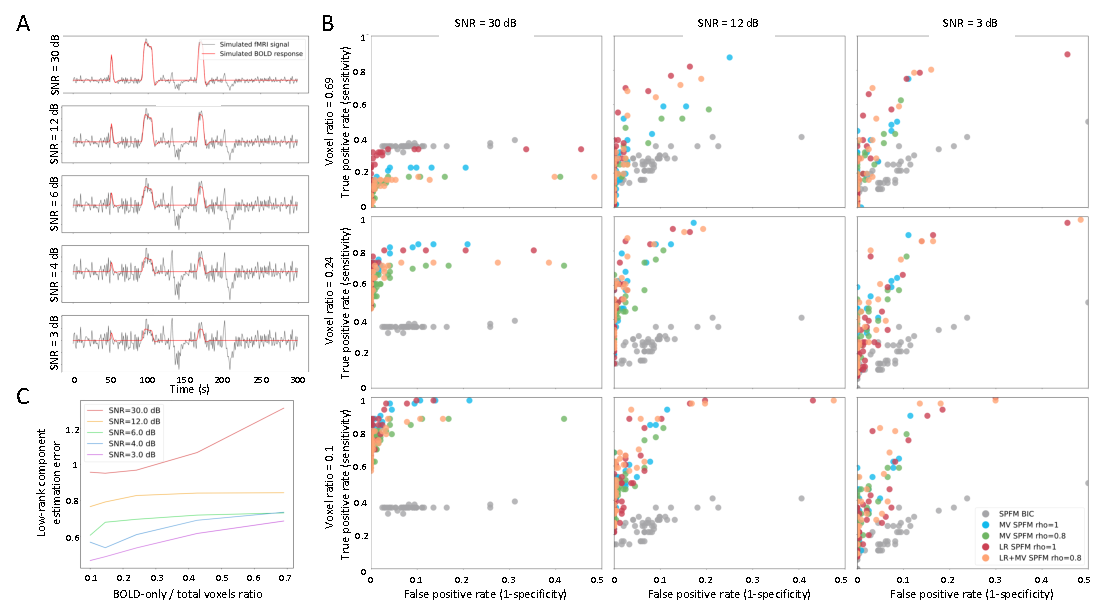
\includegraphics[width=\textwidth]{figures/low_rank/figure_1_v6.pdf}
    \caption{Simulation results. A) An example of the simulated signals for the
    different SNR conditions; B) ROC values for the estimation of
    the neuronal-related signal with: SPFM using BIC (SPFM BIC),
    SPFM with no low-rank estimation and no spatial regularization (SPFM,
    $\rho=1$), MV-SPFM with no low-rank estimation (MV-SPFM, $\rho = 0.8$), the
    SPLORA-PFM algorithm with only the L1-norm (LR+SPFM, $\rho=1$), and the
    SPLORA-PFM algorithm ($\rho = 0.8$). C) Estimation error of the low-rank
    components for different ratios of BOLD/total number of voxels.}
    \label{fig:low_rank_1}
\end{figure*}

\cref{fig:low_rank_1}B depicts the receiver operating characteristic (ROC)
curves with the sensitivity and specificity rates for the estimation of the
neuronal-related signal $\mathbf{\hat{S}}$ for each simulation scenario.
Regardless of the simulated SNR and the BOLD/total voxels ratios, the ROC values
demonstrate the proposed SPLORA-PFM algorithm achieves higher specificity and
sensitivity than the original SPFM method, except for the highest BOLD/total
number of voxels ratio and highest SNR where the multivariate nature of the
model prevents the algorithm from fitting accurately each voxel. As expected,
all variations of the proposed algorithm exhibit lower sensitivity as the SNR is
reduced while maintaining the level of specificity. In addition,
\cref{fig:low_rank_1}C plots the error of the low-rank component estimate
obtained with the SPLORA-PFM algorithm for $\rho = 0.8$, showing that its
estimate improves with a lower BOLD/total voxels ratio.

\subsection{Experimental Data}

\begin{figure*}[th!]
    \centering
    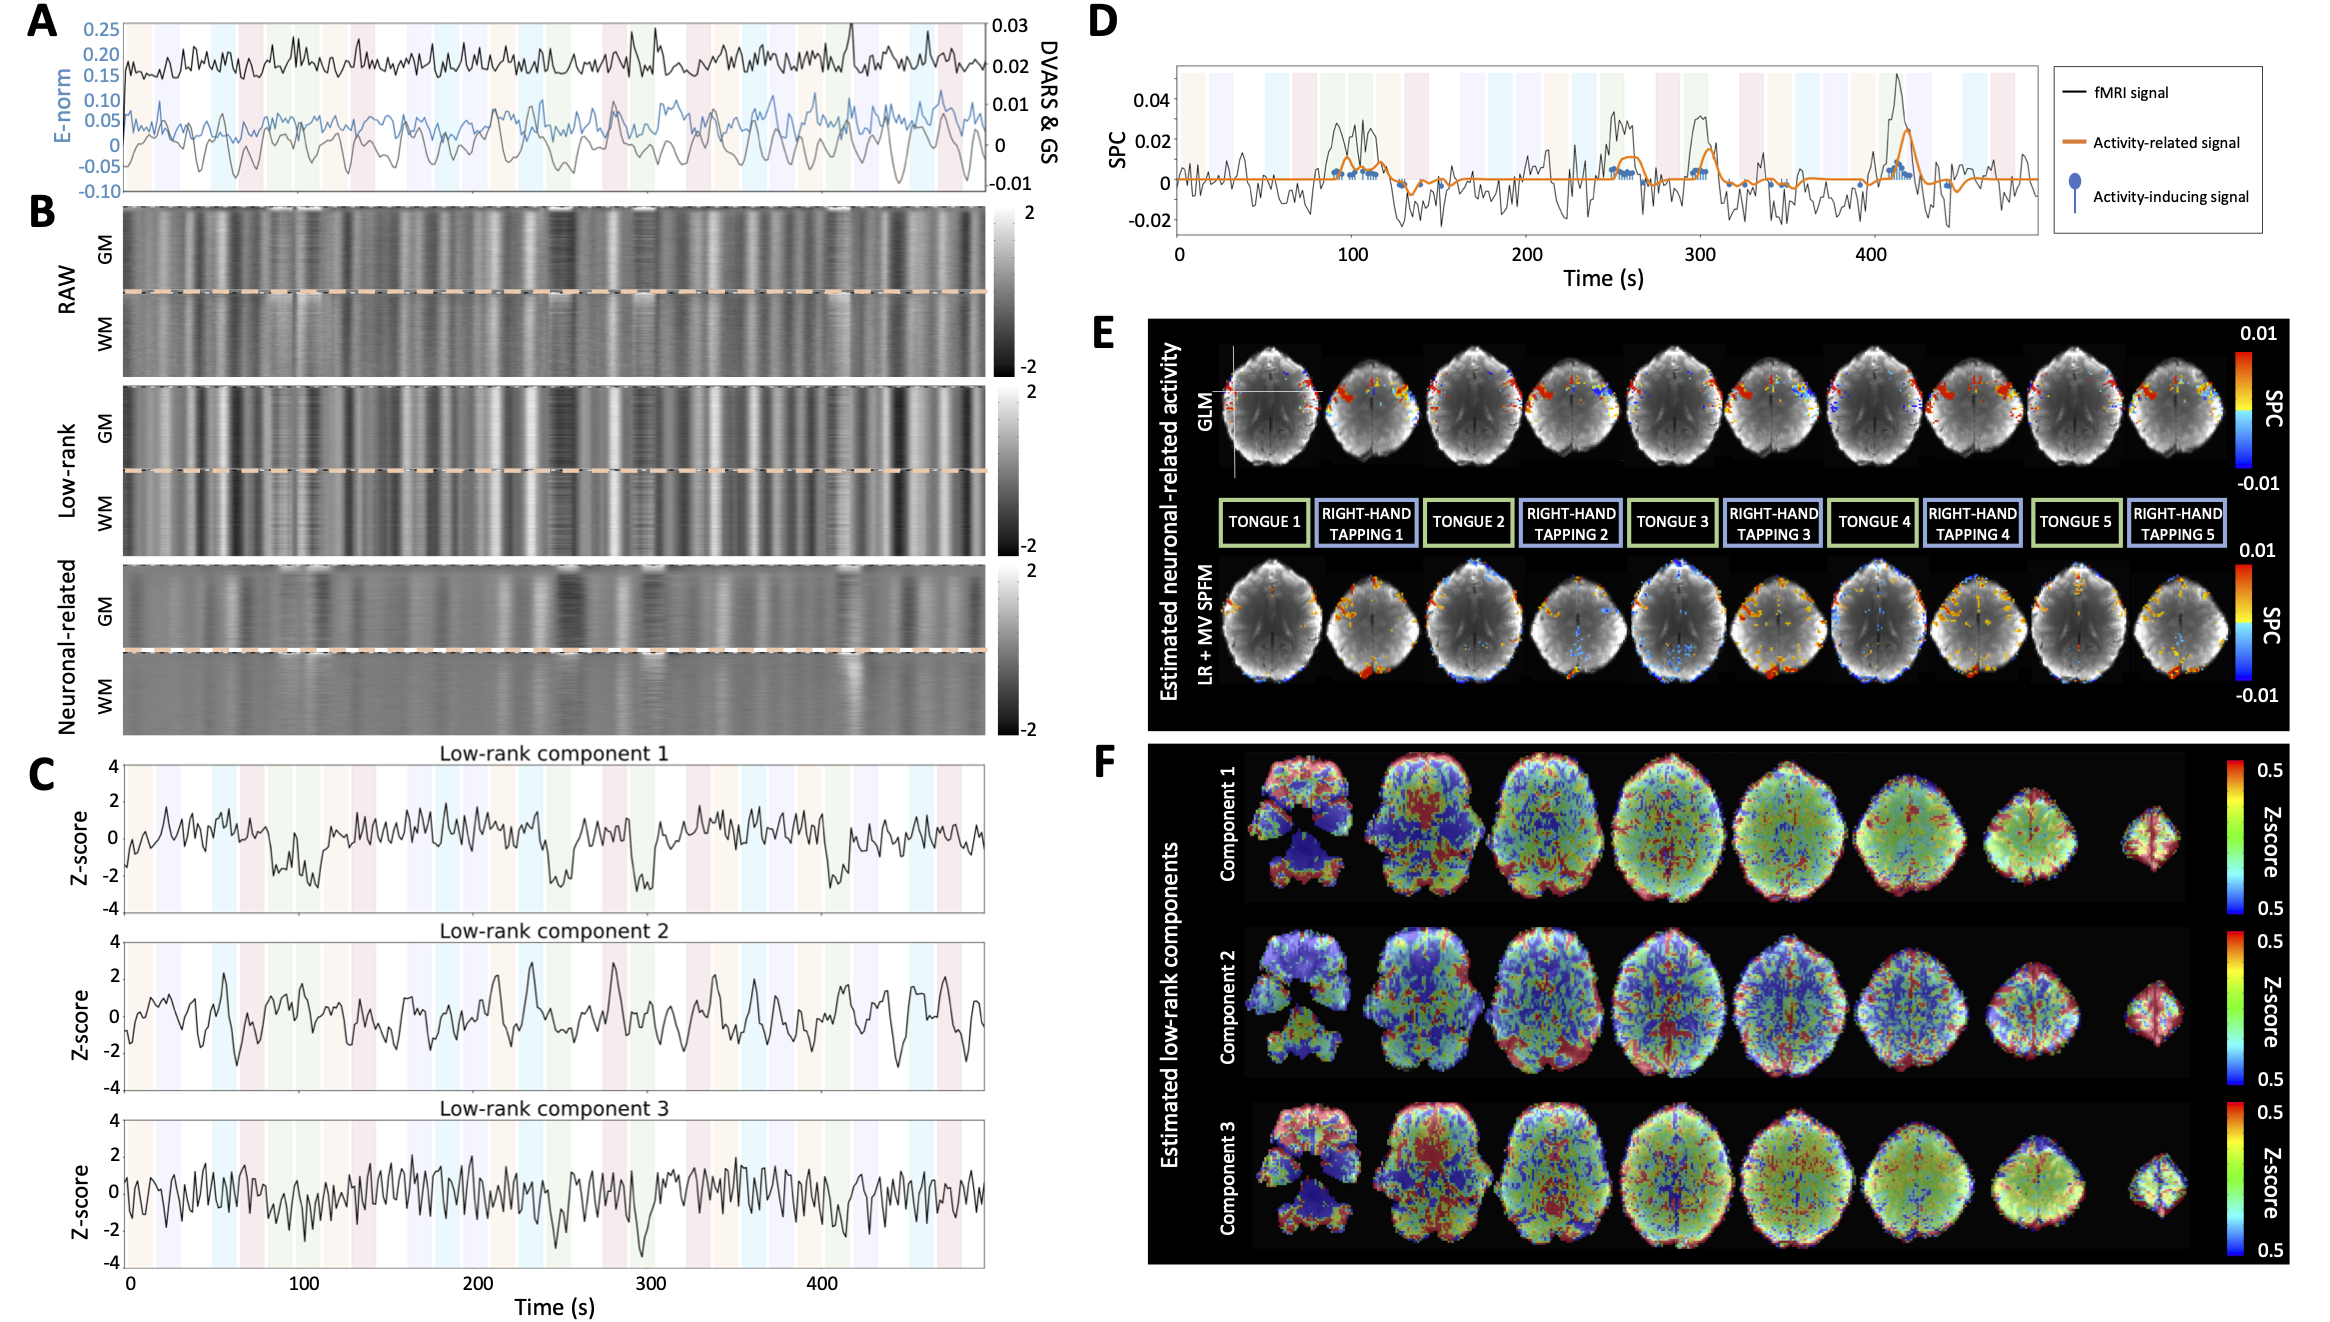
\includegraphics[width=\textwidth]{figures/low_rank/figure_2_no_G.pdf}
    \caption{A) Euclidean norm of the motion displacements (E-norm) (blue),
    DVARS (black) and global (gray) signals of the fMRI data; B) Grayplots of
    gray matter (GM) and white matter (WM) of the preprocessed fMRI
    data, the estimated low-rank and neuronal-related components; C) Time series
    and F) maps of the estimated low-rank components; D) Time series and E) maps
    of representative single-trial neuronal-related (motor) activity. The color
    bands in the plots with the time series illustrate the timing of the
    different conditions.}
    \label{fig:low_rank_2}
\end{figure*}


\begin{figure*}[th!]
    \centering
    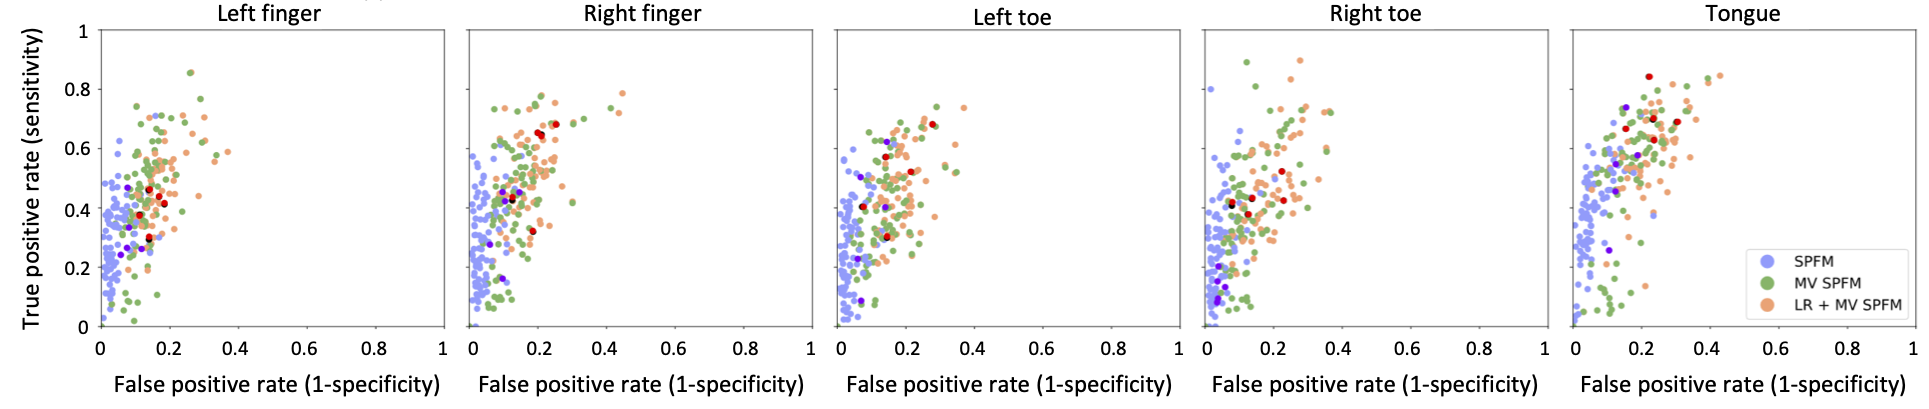
\includegraphics[width=\textwidth]{figures/low_rank/figure_3.pdf}
    \caption{ROC values of the five conditions for the three algorithms tested:
    SPFM, MV-SPFM and SPLORA-PFM (red, dark-purple and dark-green dots
    correspond to the subject in \cref{fig:low_rank_2}).}
    \label{fig:low_rank_3}
\end{figure*}


\cref{fig:low_rank_2}A-F depict the results of the SPLORA-PFM algorithm in a
representative dataset. For this subject and session, the proposed method
estimated $P=3$ global low-rank components whose time series $\mathbf{a}_p$ and
spatial maps $\mathbf{v}_p$ are shown in Figures 2C and 2F, respectively.
\cref{fig:low_rank_2}A shows the Euclidean norm of the motion displacements
(E-norm), DVARS (the spatial root mean square of the data;
\cite{Smyser2011FunctionalconnectivityMRI,Power2012Spurioussystematiccorrelations})
and the average global signal (GS) time series, whereas \cref{fig:low_rank_2}B
displays the grayplots of the preprocessed data (RAW), estimated low-rank
component and estimated neuronal-related component in gray matter (GM) and white
matter (WM) voxels. The first low-rank component captures signal fluctuations
related to head movements and susceptibility artefacts during the 'moving the
tongue' condition, suggesting that the subject moved the head while performing
the tongue movement task. The second low-rank component has a time series that
closely follows the global signal and its spatial map actually delineates major
arteries and draining veins, whereas the third component is clearly related to
widespread physiological fluctuations. Among participants, the number of
estimated low-rank components ranged between 1 and 5.

Furthermore, \cref{fig:low_rank_2}D and \cref{fig:low_rank_2}E illustrate the
time series of the estimated neuronal-related signal for a representative voxel
(see cross in the first map) and the maps for several individual events of the
tongue movements and right hand finger tapping conditions, respectively. The
SPLORA-PFM maps reveal clusters of activity in similar regions to those inferred
with a traditional general linear model (GLM) analysis, which is aware of the
timings of the events. The single-trial GLM activation maps are thresholded
based on their t-statistic at a significance threshold of $p < 0.001$. Notably,
the SPLORA-PFM maps still depict the tongue areas of the motor cortex
bilaterally even though the timing of the first low-rank component also closely
followed the tongue condition.

Finally, \cref{fig:low_rank_3} depicts the ROC values of the MV-SPFM and
SPLORA-PFM, both using $\rho=0.8$, and the original SPFM algorithm using the GLM
maps of each event thresholded at a $p = 0.001$ as the ground-truth. The ROC
curves of the five motor task conditions show that both the MV-SPFM and the
SPLORA-PFM approaches provide higher sensitivity at the cost of a reduced
specificity, and that the higher complexity involved in estimating the low-rank
component does not diminish the accuracy in deconvolving the neuronal-related
component of the signal. 

This work introduced a novel formulation for the deconvolution of BOLD fMRI data
using a low rank and sparse algorithm that captures global fluctuations due to
motion artefacts or physiological signals that typically reduce the accuracy of
neuronal related estimates of currently used algorithms. The formulation
described in this chapter was presented for single-echo acquisition and the
spike model. However, it can be adapted straightforwardly for multi-echo
\citep{CaballeroGaudes2019deconvolutionalgorithmmulti} or the block model
\citep{Karahanoglu2013TotalactivationfMRI,Cherkaoui2019Sparsitybasedblind,Urunuela2023HemodynamicDeconvolutionDemystified}
using the multi-echo and innovation signals described in \cref{cha:multivariate}
and \cref{cha:synthesis_analysis} respectively. Likewise, the selection of the
regularization parameters $\mathbf{D}_s$, $\lambda_L$ and $\rho$ was done
empirically here and could be further optimized using robust approaches such as
stability selection
\citep{Meinshausen2010Stabilityselection,Urunuela2020StabilityBasedSparse} as
described in \cref{cha:stability} and \cref{cha:multivariate}. Finally, future
work will be directed towards evaluating the performance of SPLORA-PFM on
resting-state data. Specifically, these evaluations will assess its
effectiveness in mitigating the influence of commonly observed global
fluctuations on activity-inducing signal estimates, since it is expected that
SPLORA-PFM will exhibit superior performance in this regard compared to its
performance on task fMRI data.
